

\section{Recommender systems in general}
\index{Recommender System}
As already mentioned RS help a user finding relevant items by filtering them out.
Depending on the context these items can be of any form.
In a e-commerce context for example these items can be a selection of products a online shop has.
A item in the context of a library in contrast are book which are free to borrow.
\citep[p.~377-378]{burke:2007}

{\color{red}RS noch mal besser beschreiben (wie in der einf\"uhrung nur genauer)}
%Even though has already been a brief introduction into recommender systems a much more in depth view will follow.
When describing a RS, one also has to describe the different users and the goal they want to achieve.
On the one hand is the provider of an RS - for the time being let's assume that the provider is a huge online shop selling apparel.
On the other hand, there is the client using an offered RS to simplify the search for products best suited for his needs.
In case of a online shop the user probably wants clothing that is after his fancy and in his size.
The online shop however, pursues many more objectives.
When he offers a RS to the user, he wants to
\begin{itemize}
    \item\textbf{Increase sells}\hfill\\
        By determining and offering the items the user likes most, the chance of the user buying the praised product will increase.
    \item\textbf{Selling more diverse items}\hfill\\
        Often the user only has a vague idea of the product he wants and only knows the well-established ones.
        RS can help to recommend products he needs and he wouldn't have found otherwise.
    \item\textbf{Increase user satisfaction to gain customer loyalty}\hfill\\
        {\color{red} Explain in detail.}
        With good recommendations and a pleasing user interface the user is more likely to accept recommendations.
    \item\textbf{Increase user fidelity}\hfill\\
        A RS links the using behaviour to the users previous one.
        This helps to get a more accurate picture of the users preferences.
    \item\textbf{Gain better understanding about the users needs}\hfill\\
        When the general preferences of users are known, it is possible to adapt the internal work flow of the RS provider to the user.
        This means, that an apparel shop can increase the stock on some specific cuts/patterns or colours, since the customers will demand them.
\end{itemize}
as mentioned by \citeauthor{ricci:2011}.\citep[p.~4-5]{ricci:2011}
\\

In contrast to the RS provider the user has way more diverse objectives.
\citeauthor{herlocker:2004} defined the most common tasks a RS has to fulfill in order to suit the users needs.
\begin{itemize}
    \item\textbf{Annotation in context}\hfill\\
        Given a catalog of items a RS can highlight items from which it suggests that the user may like.
    \item\textbf{Find good items}\hfill\\
        Provide users with a list of recommended items plus a estimation of how likely the item appeals to the user.
    \item\textbf{Find all good items}\hfill\\
        In order to reduce choice overload RS filter out most of the good items which may attract the user.
        Due to the filtering it may happen that not all of the items which could please the users needs will be recommended.
        In some domains however this must not happen.
        Or to put it into search engine terminology: The recall must be as high as possible.
    \item\textbf{Recommend sequence}\hfill\\
        Instead of recommending items that fulfill all requirements on their own it is also possible to recommend a combination of items.
        Rather than a single item a composite of items will be recommended to the user.
    \item\textbf{Just browsing}\hfill\\
        It has been noticed that many user browse through website without the intention of buying items but rather looking through the assortment offered.
        In such cases a RS doesn't have to make precise recommendations, since they do not matter anyway.
    \item\textbf{Find credible recommender}\hfill\\
        Users that are aware of the fact that their search for items is supported by a recommender system tend to purposely test the recommender systems quality.
        This way they can either gain more trust towards the recommendations - if their tests are passed by the RS - or the opposite may occur.
    \item\textbf{Improve profile}\hfill\\
        In order to actively improve their user profile for a RS users may contribute to rating of items.
        Their hope is that the quality of recommendations will further raise when the RS possesses more information about their preferences.
    \item\textbf{Express self}\hfill\\
        Many recommender systems build their recommendations upon a user profile for each user that includes a rating for items.
        Some users use the possibility of rating items to express themselves and their opinion.
    \item\textbf{Help others}\hfill\\
        Some users believe that they can help the community around a certain website that uses a RS by rating and evaluating items.
        This process is also highly connected to the previous one (Express self).
    \item\textbf{Influence others}\hfill\\
        As negative side effect it has bee proven, that some users try to manipulate others by giving dishonest ratings.
\end{itemize}
(as taken from \citep[p.~13-17]{herlocker:2004})

So there are various reasons for online service provider to introduce RS as an additional service to support their business.
With this in mind research question \textbf{Q1} can be solved.
While most of the goals from the RS-provider in regard to a RS are implicitly achieved by a well-functioning RS that satisfies the user, the requirements can be defined by the users wishes.
Generally a user seems to want a RS that offers credible recommendations which are built on a transparent method he can comprehend.





\subsection{Data and knowledge sources}
\label{sec:data-knowledge-source}
Any RS needs data from which the suggested items will be calculated and most of the time information about the requesting user is also necessary.
The data heavily influences the selection of recommender algorithms which provide suggestions for the user.
\citep[p.~7-8]{ricci:2011}
RS can either work on personal or non-personal information.
Recommendations built upon personalized information use any information about the user they can get while non-personalized RS use more generic data.
%There are knowledge poor algorithms whose input data solely consists of user rankings.
%But there also so called knowledge dependent algorithms using social relationship or activities of users for instance.\citep[p.~7-8]{ricci:2011}

\subsubsection{Non-personalized recommendations}
\index{non-personalized RS}
Since personalized RS will be discussed in depth in the later sections there won't be a example yet.
Instead there is be a brief sample for a non-personalized RS and a possible data source:
\\
A common resource for information which is not individual-related are sales figures.
Items that are frequently bought in general are more likely to be of use for a generic user whose preferences remain unknown.
\citep[p.~10-11]{ricci:2011}
A common application for this concept are so called bestseller-books for bookshops or a record chart for music.
This approach is especially useful, if no other data is available or a highly sophisticated RS would be unnecessary expensive.

\subsubsection{Personalized recommendations}
\index{personalized RS}
Personalized RS, however, try to utilise as many information about a user as they can get.
Any resource a recommender can use is classified as either an item, a user, or a transaction.

\paragraph{Item}~\\
\index{item}
Items are the products that will be suggested to the user.
In the case of an apparel shop this will be clothing and maybe some products that are related such as handbags or accessory like sunglasses, etc.
For any item a complexity can be estimated.
There are factors such as its structure, textual representation, as well as time dependent importance of a product.
Even thought clothing may contain certain time-dependency (winter vs. summer season), its general complexity is rather low.
A typical high complexity item may be insurance policies, jobs, or financial investments.
Items can also be distinguished by their value and its costs.
While the value states how valuable the item is for the user, costs are the combination of monetary value of the item plus the effort to require information about and getting it.
With the complexity of a product rising, also the effort to inform oneself about it will increase.
\citep[p.~8]{ricci:2011}

\paragraph{User}~\\
\index{user}
All users differ from each other - therefore one can not simply make a recommendation which satisfies every users needs.
In order to generate a matching recommendation for a given user information about him or his preferences are necessary.
Diverse recommendation approaches use different kinds of data.
These different ways will be discussed later, in section~\ref{sec:recommenderapproaches}.
The data, however, one can collect about the user is manifold.
It ranges from demographic information such as age, size, sex, nationality/cultural background, income to his behaviour as shown in search queries or ratings for a specific kind of product.
Any of the named attributes is relevant for an online clothing store, as they determine the brand (possibly influenced by income), imprint (may depend on age), and so on.\citep[p.8-9]{ricci:2011}
It is also possible, to use item-rankings or purchase history provided by users to compare the similarity of users.\citep[p.~377-378]{pradel:2011}

\paragraph{Transactions}~\\
\label{sec:feedback}
\index{transaction}
Transaction describe the interaction between the user and the RS.\citep[p.~9]{ricci:2011}
It can be differentiated into explicit and implicit feedback from the user towards the RS.
While explicit feedback requires the users to evaluate certain items in order to get a picture of the users preferences, implicit doesn't.
Instead implicit feedback will be gained by monitoring the user.\citep[p.~76-77]{lops:2011}
So implicit feedback will be provided by the normal usage of the online shop.
This means, that every time the user interacts with a product, i.g. by viewing it, the RS learns that this product may be relevant to the user.\citep{taghipour:2007}
The interaction with the RS includes the users browsing patterns (in a web based RS), his search queries and can also involve the users mouse movement (when he uses a computer).\citep[p.~146]{koren:2011}
A online clothing store could for example use the clients search queries, how long he views a specific product.\\
In contrary explicit feedback needs the users active involvement.
The most common sources for explicit feedback are a rating whether the user likes the product or not, or a textual comment - also describing, whether he likes it nor not.
The attitude towards a product will often be retrieved through a rating.
Common ones are either binary ratings with like and dislike as possible values, or some where the user can rate a product with points, similar to grades.\citep[p.~77]{lops:2011}


{\color{red}TODO Erkl"aren abgrenzung zwischen knowledge und context}


\subsection{Different approaches}
\label{sec:recommenderapproaches}
As already mentioned there are various sources of information a recommender system can use and the choice heavily impacts the quality of recommendations.
Different algorithms are suited for different tasks and have both benefits and drawbacks in comparison to each other.\citep[p.~377-378]{burke:2007}
As knowledge has already been introduced in section~\ref{sec:data-knowledge-source} we will further focus on them.
There are four major approaches \citep[p.~378]{burke:2007} which we will discuss and adapt to the example of an online clothing shop as the final objective is to implement one.

\paragraph{Content-based}\hfill\\
\index{content-based}
Each item or product is defined by its attributes such as its colour, price, age, etc.
And each user has his own rating for each of the attributes which determine whether he likes the item or not.
Every time the user gives feedback to the RS in form of preferring or rejecting an item the RS will adapt its information about the users preferences of the items attributes.
The RS determines items it can recommend to the user by comparing each of the items attributes with the users preference.
\citep[p.~75]{lops:2011}\\
In reference to a clothing store every product can be defined through its colour, brand, price, pattern and so on.
Every user however, has his very own rating for each of the attributes.
The closer all attributes of an item match the preference of a user, the higher is the probability that the user likes the item.
A content-based approach will be implemented and further described in section~\ref{sec:implementation-contentbased}.
As recommender algorithm Rocchio's algorithm will be used (section~\ref{sec:rocchio}).
\\
However this approach has a major drawback.
Every new user who has no purchase history or anything else that indicates preferences leads to a \index{cold-start problem} cold-start problem.
The cold-start problem describes a situation in which a RS has not sufficient information about a user to make credible and useful recommendations.
A content-based RS encounters a cold-start situation for every new user it has to provide with recommendations.
\citep[p.~378-379]{burke:2007}

\paragraph{Collaborative filtering}\hfill\\
\index{collaborative filtering}
The idea of collaborative filtering is based on similarity of users.
Two Users which are similar in their preferences are more likely to predict useful items for each other.
In order to determine which users have similar opinions towards the items, their item-ratings are being compared.
\citep[p.~291-292]{schafer:2007}
Within an online clothing store this can be achieved by introducing a rating system for clothing.
When all users give their opinion about the clothes for every user a matching partner can be found.
Assuming that there are two user (user $A$ and user $B$) with similar preferences, preferred clothings from $A$ can be suggested to $B$ if $B$ hasn't evaluated the piece of clothing yet.
\\
RS based on collaborative filtering also encounter cold-start problems.
A cold-start situation expresses itself for items without any user rating.
In order to recommend a item to a user it must be rated by others.
But if there is no rating available, it simply cannot be recommended to any user.
\citep[p.~378-379]{burke:2007}
%Similiar to the content-based approach these RS require information about customer preferences in order to find users with similiar behaviour and likings.
%New users however have no purchase history or haven't given any information about their preferences yet.
%Therefore they cannot be assigned to any other users which makes it hard to provide good recommendations.

\paragraph{Demographic}\hfill\\
\index{demographic}
These systems rely on demographic data which is available for every user.
Assumptions about user preferences are build upon the assumption, that the users demographic profiles provides enough information to estimate his preferences.
Demographic data can consist of the users age, sex, nationality/cultural background, income, etc.\citep[p.~12]{ricci:2011}
Income for instance can give information whether clothing of well-known brands is appropriate or not.
\\
While collaborative filtering and content-based approaches learn with every of the users steps demographic approaches require initial data about a user - namely demographic data.
This leads to another kind of cold-start problem where there is - once again - not sufficient information about a user available.
In contrast to a purchase history as required by collaborative filtering for example it can be easier to obtain demographic data by simply questioning the user about it.

\paragraph{Knowledge-based}\hfill\\
\index{knowledge-based}
Knowledge-based approaches rely on domain-knowledge about items and need additional information about the users needs.
\citep[p.~12-13]{ricci:2011}
If it's known that a given users goes for a hiking trip, it would be good to recommend him clothing associated with outdoor activities.
This could be items such as a raincoat or hiking boots.
\\
While knowledge-based approaches do not encounter any cold-start problematic, they do not scale well in long-term application.
Since they do not have any learning-component, they can not adapt to the users future needs as they may evolve with time passing.
Therefore their recommendations quality will be surpassed by another learning recommender system, similar to one based on collaborative-filtering, when information about the user is available.
\citep[p.~12-13]{ricci:2011}

\begin{figure}[h]
    \center
    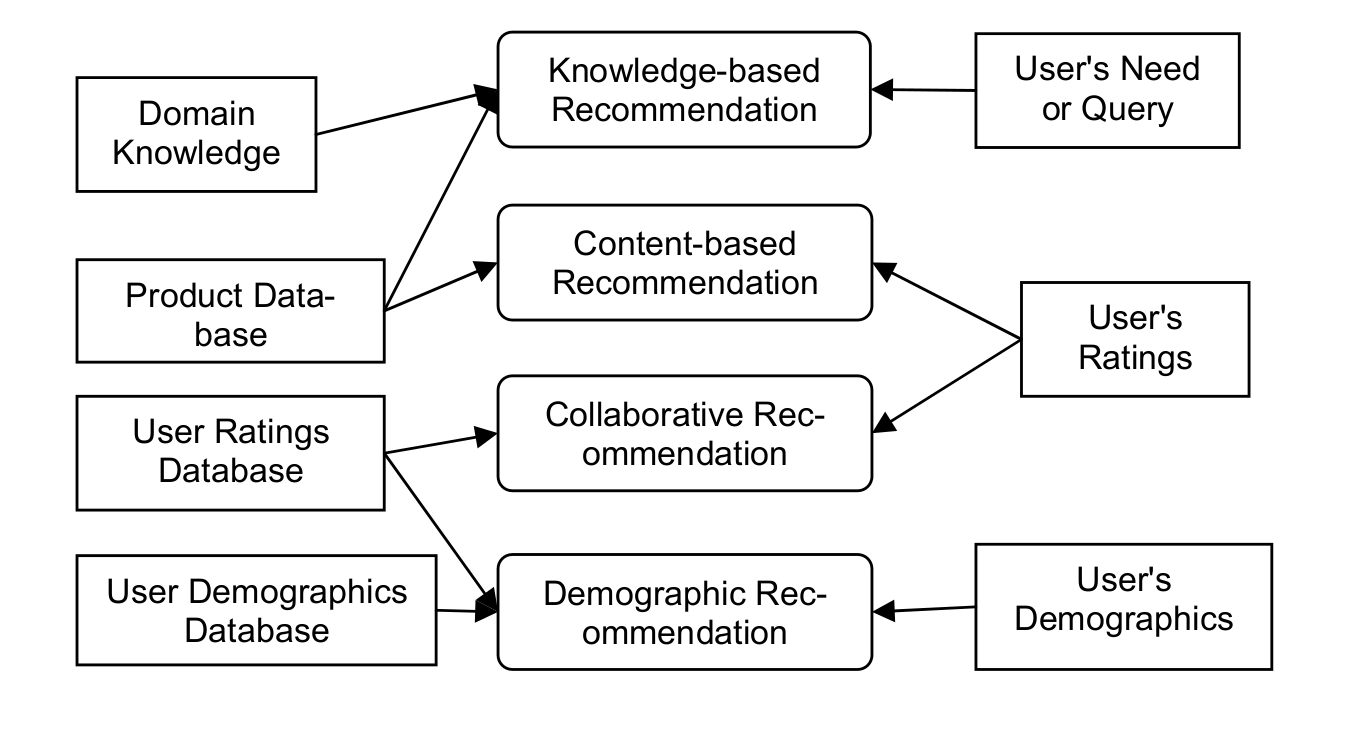
\includegraphics[scale=0.3]{inc/recommendersystems/RecommendationTechniquesAndKnowledgeSources.png}
    \caption{Recommendation techniques and their knowledge sources.\citep[p.~379]{burke:2007}}
\end{figure}

\paragraph{Hybrid systems}\hfill\\
\index{hybrid recommender systems}
As already mentioned learning-based techniques (such as collaborative-filtering, content-based, demographic) are affected by cold-start problems.
Knowledge-based techniques however are not, but have other problems.
And as stated by \citeauthor{herlocker:2000} recommender technologies do not compete, but can rather increase their overall performance when they are being combined.\citep[p.~241]{herlocker:2000}
In order to overcome these problems these approaches can be combined.
This way drawbacks of one approach can be nullified by combining it with another and vice versa.
There are various ways multiple recommender approaches can be mixed together - however that's out of scope for this thesis.
\citep[p.~378-380]{burke:2007}
There have alreaby been studies about hybrid recommender systems and which approaches work best with which.
The bottom-line of a study done by \citeauthor{burke:2007} indicates that hybrid RS achieve good results and are promising.
And it appears that the combination of knowledge-based recommender systems and others result in very good recommendations.
\citep[p.~405-406]{burke:2007}
\\

\noindent
As knowledge-based RS in combination with other seem to deliver good results the best RS approach for recommending clothing based on implicit feedback might be a content-based or collaborative-filtering approach supported by a knowledge-based RS.
Especially taste in fashion changes itself in a rather short-term way.
Therefore a learning RS method that adapts to the users shifts in taste would be best in order to guarantee useful recommendations.
Knowledge also comes useful as seasons heavily impact the variety of apparel that is beeing bought.
Therefore a hybrid RS mixing up knowledge with a content-based or collaborative filtering approach might be best for a online-shop that utilizes implicit feedback what's also the answer to \textbf{Q2}.
%Learning, as explained for content-based and collaborative-filtering approaches, can be used to adapt the RS results to changes in the users taste in fashion or changes in fashion trends.
%In some cases collaborative-filtering methods might not be the best choice for recommendations in the context of apparel, because some individuals tend to buy clothing for different persons.
%This is especially true for parents who buy clothing for their children.\citep[p.~22]{hackenberg:2011}
%Since content-based and collaborative filtering approaches learn while the clothing taste of a user and
% verbessern der ergebnisse mit knowledge (saisons, etc.)

%\subsection{Critics on RS}
%{\color{red}Bei Onlinezeitungen: Nutzer bekommen nur noch Artikel die sie lesen wollen --> verdummung? Wenn man nicht weis woher die empfehlungen kommen --> creepy (windows10) (Explaining Collaborative Filtering Recommendations)}
